\documentclass[../main/TOP_manual]{subfiles}

\begin{document}

\chapter{TOP structure and workflow}
\label{chap:ModDes}

TOP is the NEMO hardwired interface toward biogeochemical models, which provides the physical constraints/boundaries for oceanic tracers (Fig. ~\ref{fig:topstructure}).

Based on a modular structure, this component allows one to exploit available built-in modules and further develop a range of applications, spanning from the implementation of a dye passive tracer to evaluate dispersion processes (by means of MY\_TRC), track water masses age (AGE module), assess the ocean interior penetration of persistent chemical compounds (e.g., gases like CFC or even PCBs), up to the full set of equations to simulate marine biogeochemical cycles.

TOP interface has the following location in the code repository : \path{<nemo-repository>/src/TOP/}

and the following modules are available:

%-----------  tableau  ------------------------------------
\begin{itemize}
        \item \textbf{TRP}    	 :    Interface to NEMO physical core for computing tracers transport
        \item \textbf{CFC}	 :    Inert tracers (CFC11,CFC12, SF6)
        \item \textbf{C14}	 :    Radiocarbon passive tracer
        \item \textbf{AGE}	 :    Water age tracking
        \item \textbf{MY\_TRC}   :    Template for creation of new modules and external BGC models coupling
        \item \textbf{PISCES}    :    Built in BGC model. See \cite{aumont_2015} for a complete description
\end{itemize}
%----------------------------------------------------------

\begin{figure}[ht]
\begin{center}
\vspace{0cm}
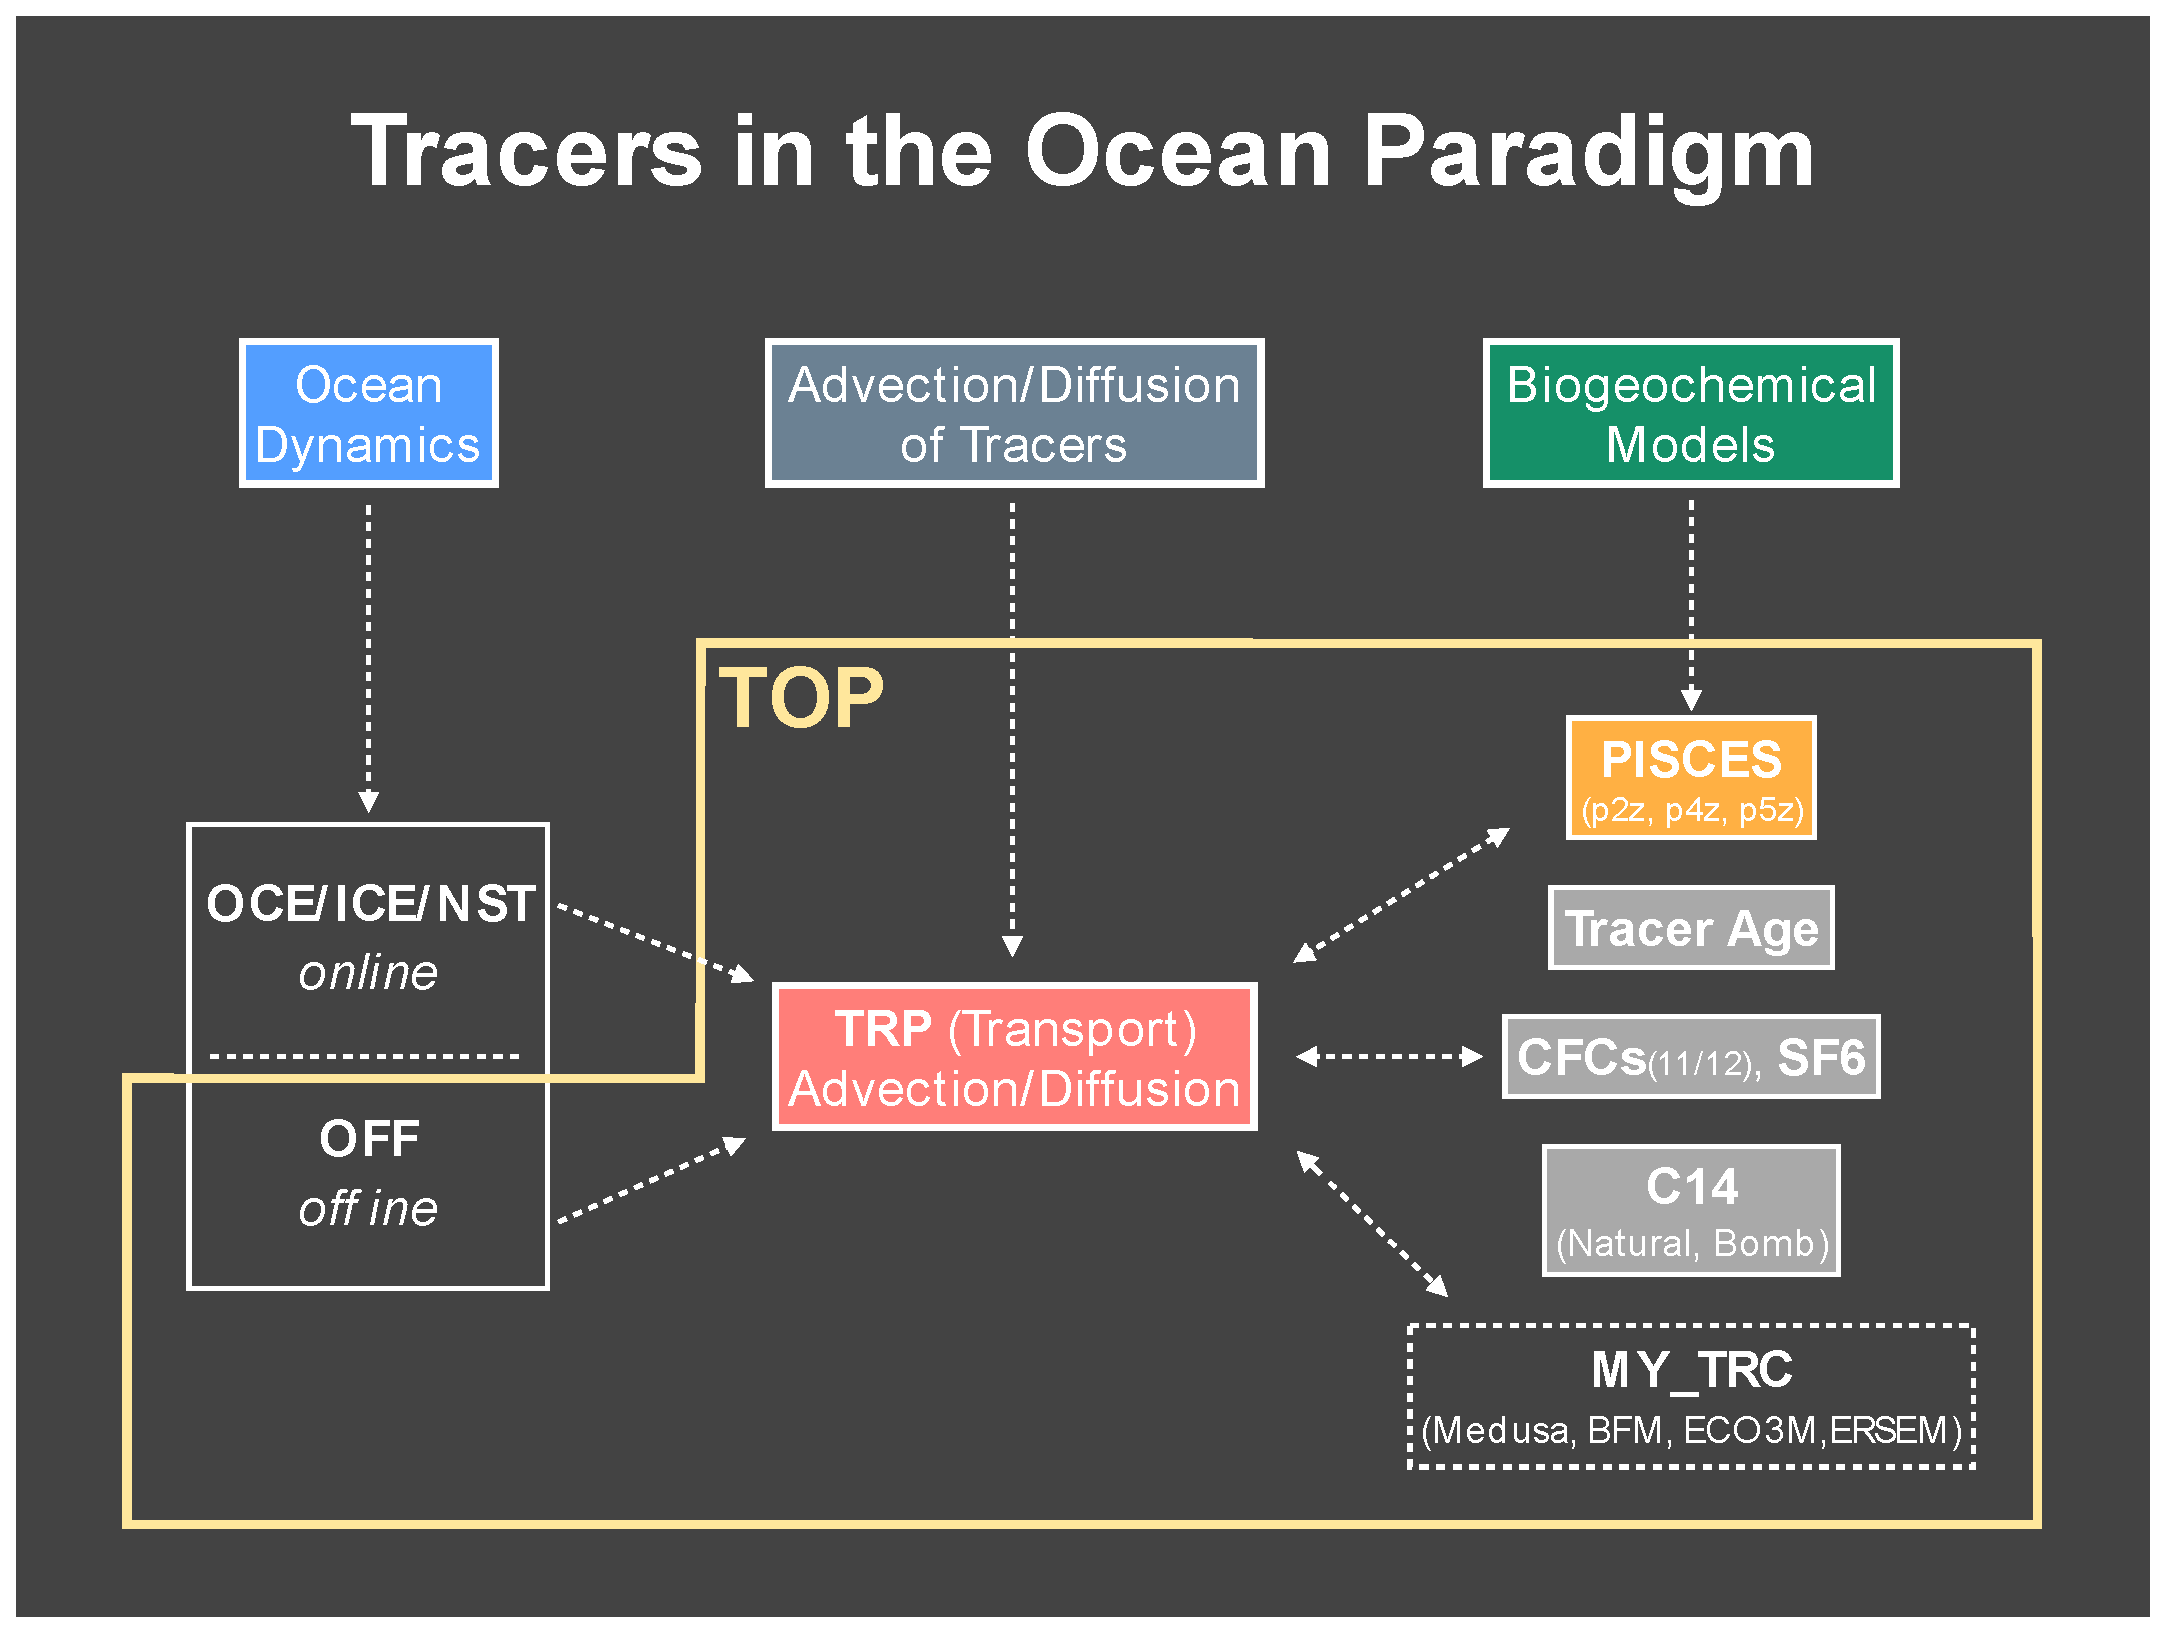
\includegraphics[width=0.70\textwidth]{Fig_TOP_design}
\caption{Schematic view of the TOP interface within NEMO framework}
\label{fig:topstructure}
\end{center}
\end{figure}

\pagebreak

% the following figures are screenshot of the mermaid plot genereted when accessing TOP/figures/workflow.md within gitlab
% this plots should be rewritten, e.g., using tikz graphic package

The workflow of the TOP interface within the NEMO framework is organized around two main blocks of the code, the initialization (\autoref{fig:topinit}) and time marching or "stepping" (\autoref{fig:topstep}) procedures.\\

The initialization (\forcode{trc_init}) of passive tracers variables and parameters include reading namelist, set initial tracer fields (either read restart or read data), and specific initialisation for each SMS module.

%tikz common preamble
\tikzstyle{process} = [rectangle, minimum width=1cm, minimum height=1cm, text centered,  align=center, draw=black, fill=orange!20]
\tikzstyle{line} = [thick,-,>=stealth]
\tikzstyle{arrow} = [thick,->,>=stealth]

\newcommand*{\connectorH}[2]{
  \draw[arrow] (#1) -- ++(1.cm,0) |-  (#2);
}

% initialization workflow
%
\begin{figure}[ht]
\begin{center}
\vspace{0cm}

\begin{tikzpicture}[node distance=1.5cm and 1cm]

\node (main) [process, xshift=0 cm] 
    {nemo\verb!_!init \\ (nemogcm.F90) \\ NEMO General Initialisations};
\node (ini) [process, yshift=-3.5cm, xshift=3.5cm] 
    {trc\verb!_!init \\ (trcini.F90) \\ TOP Initialisation};
\node (ini1) [process, yshift=-0.5cm, xshift=11cm] 
    {trc\verb!_!nam  (trcnam.F90)\\ initialize TOP tracers and run setting};
\node (ini2) [process, yshift=-2cm, xshift=11cm] 
    {trc\verb!_!ini\verb!_!sms \\ initialize each SMS sub-module};
\node (ini3) [process, yshift=-3.5cm, xshift=11cm] 
    {trc\verb!_!ini\verb!_!trp \\ initialize transport for tracers};
\node (ini4) [process, yshift=-5cm, xshift=11cm] 
    {trc\verb!_!ice\verb!_!ini \\ initialize tracers in seaice};
\node (ini5) [process, yshift=-6.5cm, xshift=11cm] 
    {trc\verb!_!ini\verb!_!state \\ set initial state from restart or inputdata};

\draw [arrow] (main.south) |-  (ini.west);
\connectorH{ini.east}{ini1.west}
\connectorH{ini.east}{ini2.west}
\connectorH{ini.east}{ini3.west}
\connectorH{ini.east}{ini4.west}
\connectorH{ini.east}{ini5.west}

\end{tikzpicture}

\caption{TOP interface initialization workflow}
\label{fig:topinit}
\end{center}
\end{figure}


In the time-marching procedure of the model (trc\_stp), trends are computed for all tracers in relation to biogeochemical processes (source minus sinks of each TOP sub-module), 
physical transport (advective \& diffusive, forcing and boundary conditions) and output is managed using the I/O library XIOS.


% stepping workflow
%

\renewcommand*{\connectorH}[2]{
  \draw[arrow] (#1) -- ++(2.cm,0) |-  (#2);
}


\begin{figure}[ht]
\begin{center}
\vspace{0cm}

\begin{tikzpicture}[node distance=1.5cm and 1cm]

\node (main) [process, xshift=0 cm] 
    {trc\verb!_!stp \\ (trcstp.F90) \\ TOP time marching};
\node (wri) [process, yshift=-2.25cm, xshift=3.5cm] 
    {trc\verb!_!wri \\ (trcwri.F90) \\ call XIOS for output of data};
\node (sms) [process, yshift=-4.25cm, xshift=3.5cm] 
    {trc\verb!_!sms \\ (trcsms.F90) \\ BGC trends of each sub-module};

\node (trp) [process, yshift=-6.25cm, xshift=3.5cm] 
    {trc\verb!_!trp \\ (TRP/trctrp.F90) \\ compute physical trends};
\node (ini1) [process, yshift=-2.5cm, xshift=13cm] 
    {trc\verb!_!bc  (trcbc.F90)\\ surface and coastal BCs trends};
\node (ini2) [process, yshift=-4cm, xshift=13cm] 
    {trc\verb!_!dmp (TRP/trcdmp.F90)\\ tracer damping};
\node (ini3) [process, yshift=-5.5cm, xshift=13cm] 
    {trc\verb!_!ldf  (TRP/trcldf.F90)\\ lateral diffusion};
\node (ini4) [process, yshift=-7.0cm, xshift=13cm] 
    {trc\verb!_!zdf (TRP/trczdf.F90) \\ vertical mixing  after tracer};
\node (ini5) [process, yshift=-8.5cm, xshift=13cm] 
    {trc\verb!_!aft (TRP/trcatf.F90) \\ time filtering of 'now' tracer fields  \\ (Lateral Boundary Conditions called here)};
\node (ini6) [process, yshift=-10.0cm, xshift=13cm] 
    {trc\verb!_!rad (TRP/trcrad.F90) \\ Correct artificial negative concentrationst};

\node (rst) [process, yshift=-8.25 cm, xshift=3.5cm] 
    {trc\verb!_!rst \\ (trcrst.F90) \\ write restart files};

\draw [arrow] (main.south) |-  (wri.west);
\draw [arrow] (main.south) |-  (sms.west);
\draw [arrow] (main.south) |-  (trp.west);
\draw [arrow] (main.south) |-  (rst.west);

\connectorH{trp.east}{ini1.west}
\connectorH{trp.east}{ini2.west}
\connectorH{trp.east}{ini3.west}
\connectorH{trp.east}{ini4.west}
\connectorH{trp.east}{ini5.west}
\connectorH{trp.east}{ini6.west}

\end{tikzpicture}

\caption{TOP interface time-marching workflow (called by stp in \forcode{OCE/step.F90}}
\label{fig:topstep}
\end{center}
\end{figure}

\end{document}
